\chapter{Introduction}
For this thesis, I investigate the self heating of dust produced in the Basic Oxygen Steelmaking (BOS) process. The dust is a by-product of the BOS process; created by blowing oxygen  at supersonic velocities on liquid steel \cite{Ray19}. The dust is collected and compacted into a filter cake which is then stockpiled. The stockpiles provide \\ 
The temperature distribution within these stockpiles is of interest. The self-sintering process that occurs inside them are still being investigated. 
One belief is that the self-sintering process is a result of the oxidation of Iron \cite{Ray19}. There is uncertainty in the conditions that result in the stockpiles igniting; some of the stockpiles ignite and some do not. There is currently no method for predicting which stockpiles will ignite and which ones won't.  Understanding these reactions and how they affect the overall temperature will assist in developing a greater understanding of the sintering process. 
\section{Aims and Objectives}
The aim of this thesis is to develop a three dimensional model to aid in the understanding of the self sintering process in large stockpiles. To do this we look to:
\begin{itemize}
\item Determine which factors need to be included, and which can be excluded.
\item Identify the kinetics of the reactions that are occurring inside the stockpiles.
\item Understand how the construction of the stockpiles can affect their propensity to ignite.
\item Assess the kinetic model by using it to simulate experiment and comparing the results. 
\item Explore the stochastic effects of random variation in the stockpile and weather conditions.
\end{itemize}
\section{Significance}
The self sintering of BOS filter cake improves the recyclability of the material. The sintering process improves the structure of the material and as such increases its potential use \cite{Ray19}. This provides a large environmental benefit. The sintered material has higher strength, better transport properties, and larger particle size. This enables it to be recycled, as a coolant, reducing the amount of material ending in landfill \cite{Ray19}. Furthermore, this study highlights key financial benefits for the industry. If more can be done to understand this sintering process, then the material can be recycled at a lower cost. The Iron in the filter cake is of reasonable value. If there is more control over the ignition of these stockpiles then this provides a way of controlling the form of the iron so that the value can be realised. \\
%This thesis also has significance to applied mathematics. 
In these stockpiles we wish to promote the oxidation of Iron. This is uncommon in the spontaneous combustion literature. 
Much of the work on has been to prevent the combustion, as such, the models required for understanding how to promote ignition, have not been highly developed.

\begin{figure}[h!]
\centering
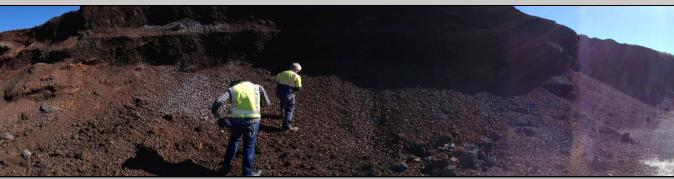
\includegraphics[scale=0.8]{figures/pile.jpg}
\caption{One of the stockpiles at the site.}
\end{figure}